This chapter provides insights into the domains of personal financial management and technology for the home which constitute the main areas of interest in our thesis. The purpose is to create a general foundation…

\section{Designing Technology for the Home}
The home is a dwelling place where inhabitants find refuge and safety; it is a place of security and protection where everyday cares fade and the things and people that one loves become the focus. It establishes a sense of belonging somewhere in the world and can have various physiological influences on the inhabitants, ranging from behavioral and emotional to even affect the overall mental health \cite{boutruche2008raising}. Designing technology for this context requires an understanding of the home as a “lived in” environment where technology is used and integrated in numerous ways and where many different activities are undertaken. The home is a messy place where rooms often have multiple purposes and are configured by the inhabitants to fit their routines and specific needs. The challenges of designing for this context stand in stark contrast to the ones faced in the work sphere where information technology has been widely used for decades. Technology for the work sphere focuses on dedicated support of particular work activities that are isolated from the environment in which the systems are placed. As a consequence, the design techniques have focused on supporting the construction of dedicated systems for particular kinds of work rather than a broader consideration of the system and the space which it is used in \cite{hughes1998understanding}. For this reason, we must be careful not to use the familiar concepts derived from the workplace when designing for the home as there is a risk of migrating a set of values that may be inappropriate for the domestic context \cite{crabtree2003finding}. As Gaver phrases it \cite{gaver2001designing}:

\tquote{There is a danger that as technology moves from the office into our homes, it will bring along with it workplace values such as efficiency and productivity at the expense of other possibilities.}{Gaver, 2001}

Intuitively we know that the workplace and home are indeed very different domains, but the challenge is not simply one of understanding this, rather it is one of developing insights into how the home is different in order to create technologies that are fitting and appropriate to the setting. Hughes et al. have investigated the role of technology in the domestic environment with a focus on the home as a “lived space” and how technology can be “made at home” in such a setting \cite{hughes1998understanding}. They found an important theme to be the aesthetic character of the home, as it is an essential part of the transformation of a house into a home. Inhabitants work at their houses by decoration and configuration in order to make them into homes and these aesthetically focused “home making” activities are of great importance to them as they encompass choices that reflect both personality and lifestyle. This emphasizes that the aesthetics are not to be taken lightly when designing technology for the home; it might even be a prerequisite that it is deemed aesthetically pleasing to be considered let into the home. However, there is a natural compromise between the aesthetic and functional traits of domestic technology. The more crucial the functionality is considered to be, the more willing we are to compromise on the aesthetics. In this regard, it is important to be aware of the close relationship that exists between the aesthetic and practical organisation of the home as these are closely intertwined \cite{hughes1998understanding}.

\subsection{Domestic Routines}
Researchers working in the field of domestic technology have identified the everyday domestic routines as a significant and highly interesting characteristic of the context \cite{edwards2001home,crabtree2004domestic,tolmie2002unremarkable}. Tolmie et al. describe how routines essentially bind everyday life together by enabling inhabitants to take action without constantly having to reason about their activities \cite{tolmie2002unremarkable} -- routines are what makes everyday life flow:

\tquote{Routines are the very glue of everyday life, encompassing innumerable things we take for granted such that each ordinary enterprise can be undertaken unhesitatingly… Routines help provide the grounds whereby the business of home life gets done. Routines mean that people can get out the door, feed themselves, put the children to bed, and so on, without having to eternally take pause and invent sequences of action anew or open up their every facet for inspection or challenge or to constantly have to account for what they are doing with explanations or rationales.}{Tolmie et al., 2002}

Crabtree et al. have studied the routines of the home by explicating the practical action that inhabitants routinely engage in, i.e. the reoccurring sequences of practical actions \cite {crabtree2004domestic}. They found the routines related to production and consumption of communication in the home particularly interesting and have, based on these routines, constructed a set of key organizational features that may instruct the development and placement of technology in the home. The features include \emph{Ecological Habitats}, \emph{Activity Centres} and \emph{Coordinate Displays} and represent the patterns of technologically mediated activity in the home \cite{rodden2004between}. Ecological habitats are places where technological artefacts and media live and where inhabitants go to find specific resources. The artefacts are placed in these ecological habitats as a matter of routine use and are thus easily located; habitats include places such as desks, shelves and tables. Activity centres are places where artefacts are recurrently manipulated and information transformed. Ecological habitats and activity centres may be different places but can also coincide; a noticeboard may at one time be a habitat for information about important upcoming events and at another a centre where the information supports social interaction. Likewise, the desk might at one time be a habitat where books, documents and reminders live and at another a centre where reports are written and emails sent. Coordinate displays are places where artefacts and media are displayed in order for inhabitants to coordinate their activities. They are constructed at easily visible sites with the purpose to trigger practical actions such as remembering to pay a bill or buy tickets for the match. An important point here is the fact that it might not be the same person who places the reminder to pay the bill and actually takes action; the displays act as ways for the inhabitants to coordinate action. Coordinate displays may also coincide with ecological habitats or activity centres. Taking the example of the noticeboard, it may act as a display for information that enables the inhabitants to coordinate social activities. As the examples indicate, it is important to remember that even though the three organizational features are distinct, the places in which they are situated often overlap, meaning the places will take on different functions at different times. The organizational features serve as conceptual and analytic resources to help guide the placement of domestic technology so it may meet the daily needs of the inhabitants. Identification of the ecological habitats, activity centres and coordinate displays in a particular setting, thus provides insights into prime sites for domestic technology deployment \cite{crabtree2003finding}.

\subsection{Ubiquitous Computing in the Home}
The domestic environment has received a great deal of attention from the ubiquitous computing community, especially through purpose built “lab houses” that aim to explore both the potentials and shortcomings of current technology and infrastructure as well as visions of the future home e.g. \cite{kidd1999aware}. While exploring the potential of full blown ‘smart homes’ is an important endeavour, so is considering the constraints of the real world on the technologies we design. As Edwards and Grinter put it \cite{edwards2001home}:

\tquote{new homes may eventually be purpose-built for such smart applications, existing homes were not designed as such. Perhaps homeowners may decide to "upgrade" their homes to support these new technologies. But it seems more likely that new technologies will be brought piecemeal into the home; unlike the "lab houses" that serve as experiments in domestic technology today, these homes will not be custom designed from the start to accommodate and integrate these technologies.}{Edwards and Grinter, 2001}

This predicted piecemeal integration of technology into the home calls for research that complements the current holistic approach to domestic technology by considering how inhabitants might bring domestic technology into their “dumb” homes. In this regard, research has broadly focused on three different approaches to the development of interactive domestic technology \cite{rodden2003evolution}: \emph{Information Appliances} which are self-contained interactive devices with specific functionality. These are often constructed by layering interactive functionality onto existing household appliances, for example using touch screens. \emph{Interactive Household Objects} combine existing household objects with interactive capabilities to create new forms of interaction which often build upon the values associated with the existing household object. And lastly \emph{Augmented Furniture} where interactive capabilities are added to the furniture in such a way that interaction is mediated through embedded sensors detecting actions with the furniture.

\section{Personal Financial Management}
A significant amount of our daily decisions and routines are rooted in money. Everything from buying basic commodities to planning for buying a new house is weaved into our financial values and habits. Many commercial tools -- mostly apps \cite{mint,spiir,levelmoney,homebudget,moneylover} -- have been developed to support and engage people in personal finances, however the majority of these tools focus on extensive data visualization and/or economic planning which is proclaimed to fail in real-life situations \cite{snow2015fixing}. Also, since these tools are mainly deployed on multi-purpose platforms, such as smartphones or laptops, many applications are fighting for our attention once we engage with these devices and consequently users might find themselves roaming social networks, making phone calls or playing games instead of staying in touch with their finances \cite[p.~3894]{coleman2008nestegg}. Even though money is a substantial part of our life, financial management and interactions (e.g. saving, trading or buying) have not received much attention from the HCI community.
Kerber et al. created a household account book which is able to capture data from receipts using optical character recognition \cite{kerber2014towards}. This feature was used to ease the process of entering data, but aside from that their solution is not that different from today’s smartphone applications. A different and very interesting take on personal finances is the future-focused smartphone application Weekly \cite{weekly}. Based on a spending goal and daily transactions the application is able to provide users with a financial forecast, e.g. spending less money than planned results in a sunny forecast whereas spending more leads to a rainy forecast. A more physical approach to tracking finances is SmartPiggy; a smartphone-connected piggy bank which uses gamification to help users keep track of multiple saving targets \cite{stockinger2013smartpiggy}. Many similar products have been developed for commercial use \cite{ernit,kash,porkfolio} (see figure~\ref{fig:ernit-kash-porkfolio}).

\begin{figure}[h]
	\centering
	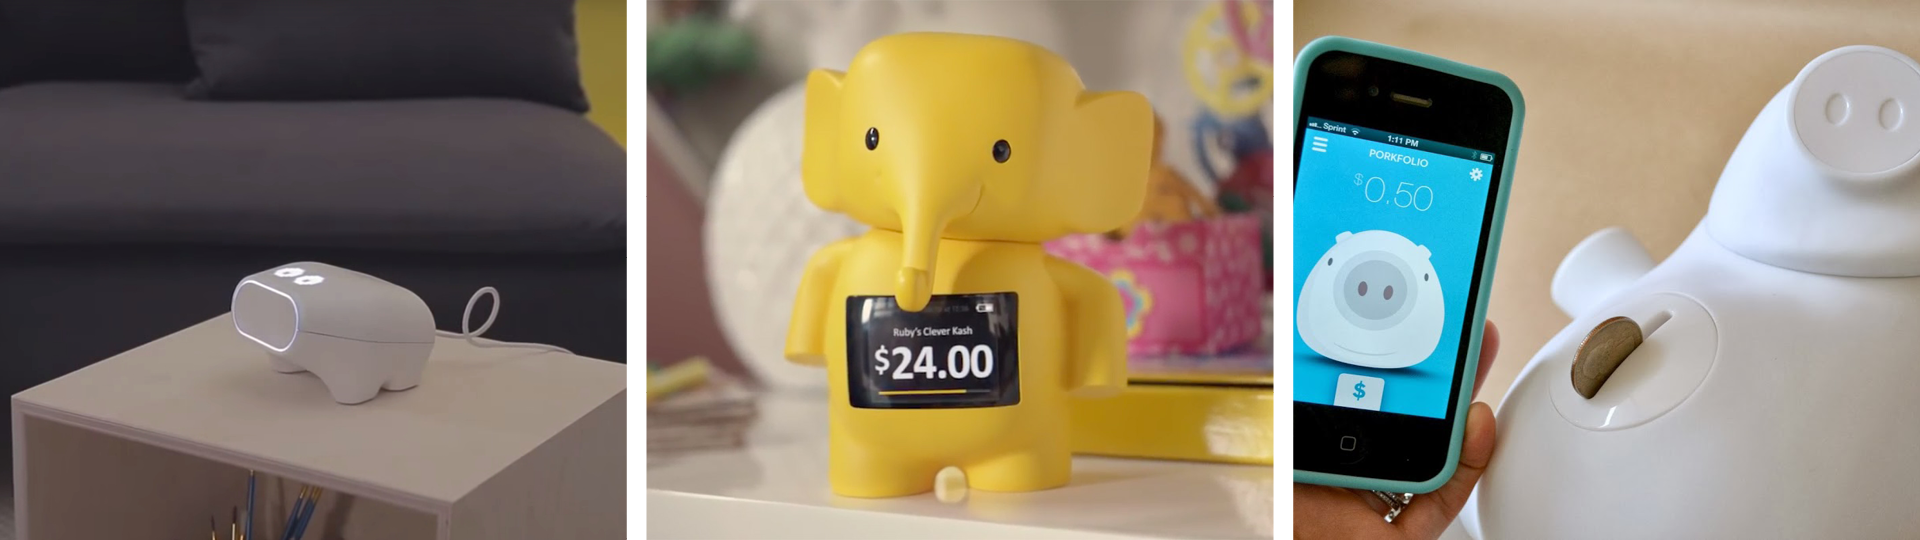
\includegraphics[width=\textwidth]{ernit-kash-porkfolio}
	\caption{Picture 1: ERNIT; Picture 2: Clever Kash; Picture 3: Porkfolio}
	\label{fig:ernit-kash-porkfolio}
\end{figure}

In 2014 Kaye et al. \cite{kaye2014money} conducted a foundational study where they investigated how people keep track of their personal finances. The study excluded financial professionals and people who systematically study finances and aimed to achieve general diversity in terms of age, income, assets, job and the presence of children and partners. In the paper the authors present three main findings: emotional reasoning for financial decisions, tools for tracking money and accounting for the unknown; the latter refers to the inability to predict future events that have an impact on personal finances and is not of interest to our project. According to Kaye et al. [ibid] most of our economic decisions are based on emotional grounds, which might not come as surprise (to some) since the notion of homo economicus, i.e. the idea that humans are self-interested actors who make economic decisions based on rational judgement, has been declared obsolete within economic theories \cite{REFERENCE}. The researchers found that people usually acted upon existing knowledge, prior experiences, worries, personal values and future dreams meaning that spendings are not always based on profit maximization or rational reasoning.
Their second finding is related to tools for tracking personal finances. In general tools were divided into two groups, namely paper systems and digital systems. The paper-based systems varied from simple index cards to more elaborate lists and calendars, and were often optimized for people’s financial focus (income, savings, stocks, etc.). Surprisingly the digital systems were not very popular. People expressed concerns regarding security and found the commercial aggregations systems (digital systems developed to provide a financial overview) somewhat frustrating mainly due to a poor user experience and lack of freedom. What is interesting here is that most people did not use a dedicated tool, however \emph{“people’s sense of their finances came from occasional glimpses at the complex whole, rather than a concerted and coherent overview of their entire situation”} \cite[p.~562]{kaye2014money} meaning that people will occasionally review the last couple of transactions and look for anything that deviates from the expected. In relation to this Kaye et al. coins the term “financial touch” which is comparable to our definition of economic awareness, however their notion also includes temporality, i.e. having ephemeral or transitory financial interactions.
By the end of the paper the researchers come with some general thoughts and observations. First of all, none of the participants seemed to use systems that integrate all aspects of a financial life, suggesting a need for rethinking existing financial systems or create new interaction experiences. The varieties of physical (paper-based) systems used also shows a great potential for more physical systems. Furthermore, personal financial management tools could also include encouraging prompts and have a more granular approach to privacy, e.g. filtering content based on who is looking.

Despite the small number of HCI studies within the area of personal financial management, Kaye et al.’s article serves as a great starting point for this thesis. They point out that financial decisions are not solely based on rational reasoning and that being aware of one’s economic state is tightly coupled to the act of observing transactions patterns and looking for anomalies. As Snow and Vyas \cite{snow2015fixing} they also highlight the misalignment between commercially available products and actual financial practices, and foresee a high potential for more physical products. As their study was carried out in America, it might not be directly applicable to the European citizens and culture, therefore, in the next section, we describe a European study that segments financial customers based on their attitude and stance towards finances.

\subsection{Segmenting Financial Customers}
\label{sec:segmenting-financial-customers}
This section presents information from a report developed by Forrester Research in 2006 \cite{ensor2006segmenting}. Although the report is more than 10 years old the data presented is still relevant today as it seeks to enlarge the traditional strategies for customer segmentation. In this thesis we will use this information as a way to understand and describe our participants’ financial motivation, behaviour and attitude.

\begin{figure}[h]
	\centering
	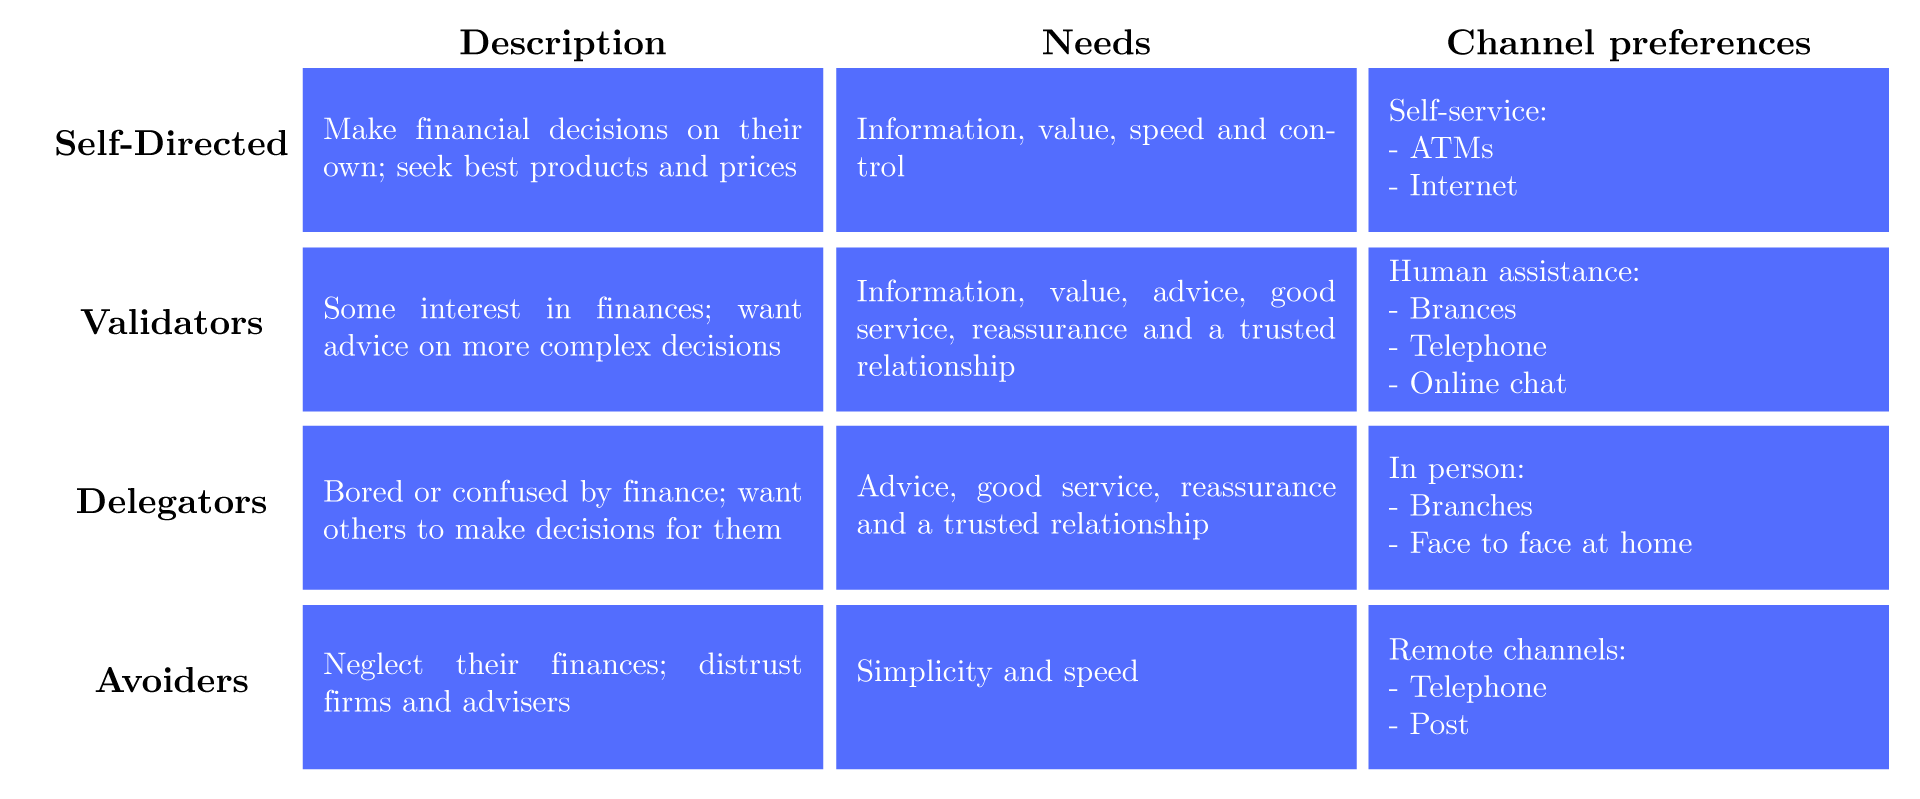
\includegraphics[width=\textwidth]{financial-customer-types}
	\caption{Types of financial customers. Courtesy to \cite{ensor2006segmenting}}
	\label{fig:financial-customer-types}
\end{figure}

According to \cite{ensor2006segmenting} the web has for many become the main source of information. Complex decisions are often based on knowledge obtained from the web and people regularly use online resources when researching for financial decision. Alongside this tendency many customers steadily adopt new service technologies leading to an increase in number of channels (phone, email, forms, etc.) used to reach the same goal. This increase is not only supported by our client’s data but it also shows that the mobile channels are on the rise compared to the more traditional platforms (see figure~\ref{fig:TO FIGURE}). To accommodate this change of behavior banks need to have an effective way of segmenting customers in order to reach a better understanding of customers’ decisions. Historically speaking customer segmentation is not new to most financial service companies, however the the current segmenting dimensions -- i.e. demographics, contribution, behaviour and attitude -- do not fully capture the complexity of customers’ behaviour. In general each dimension encompasses advantages and disadvantages, but the most useful and least ephemeral dimension is attitude since people's economic stance change relatively slowly, it is applicable to all customers and it provides a valuable insight into people’s behaviour \cite[p.~2-8]{ensor2006segmenting}. Based on financial attitude customers can be divided into four different types. They are as follows: Self-Directed, Validators, Delegators and Avoiders – an overview of each type can be found on figure~\ref{fig:financial-customer-types}.
As the name implies Self-Directed customers are highly independent and in most cases make financial decisions without consulting a financial adviser. They often have a strong interest in finances, understand financial products well and make research before making any decisions. Perhaps surprisingly, not all Self-Directed customers are willing to run financial risk for a higher return, and when it comes to more complex decisions such as pension or tax they seek advice from professionals. Compared to the other types they tend to have a better education and work full time. The second type is Validators. They have the same kind of interest in economy as the Self-Directed but lack some confidence when it comes to making decisions. For moderately complex problems the Validators seek out financial advice, but are, in comparison to the Self-Directed type, more willing to take financial risks for a higher return. Out of the four types, Validators seem to have the healthiest economy. The third type, Delegators, find finances boring and/or confusing. They would rather spend time on something else and is prepared to give up control to more knowledgeable people. When dealing with finances half of the Delegators wish to talk to other people and from a demographic perspective there is a slightly higher occurrence of women in this category. The last type is more or less oblivious to finances. Avoiders do not have much trust in financial services or advisers, and as a result they tend to neglect their finances completely. Consequently, they usually have an unhealthy economy while their lack of financial knowledge make them more risk-averse because they are not able to grasp the repercussions of their actions \cite[p.~10-11]{ensor2006segmenting}. According to the report the easiest way to spot which segment a given customer belongs to is through their behaviour, e.g. Validators are more likely to buy products through a financial adviser whereas the Self-Directed would probably do it online without consulting a professional. Furthermore, the various types seem to prefer different channels (ATM, internet, branches, etc.) and therefore this can also be used to uncover the type of a customer.

The customer segmentation and the fact that customers’ interest in personal financial matters vary a lot, needs to be taken into consideration because it will inevitably influence our findings. Hopefully, being able to make that distinction between different types of users will help us in making more informed decisions hence make better designs.
